\documentclass[a4paper,11pt]{article}
\usepackage[polish]{babel}
\usepackage[OT4]{fontenc}
\usepackage[utf8]{inputenc}
\usepackage{graphicx}

\usepackage{epstopdf}




\date{16/03/2014}


%opening
\title{PAMSI -- testowanie implementacji struktur danych}
\author{Piotr Wilkosz}

\begin{document}

\maketitle

\section{Wstęp}
Celem ćwiczenia było przetestowanie implementacji takich struktur danych jak:
  \begin{itemize}
   \item Stos --- zawierający listę lub tablicę dynamiczną
   \item Kolejka --- zawierająca listę lub tablicę dynamiczną
  \end{itemize}
Zadaniem było zmierzenie czasu wykonywania operacji wypełnienia powyższych struktor danych.
\section{Wyniki pomiarów}
\begin{enumerate}
 \item Stos bazujący na liście:
 \begin{figure}[!ht]
\centering
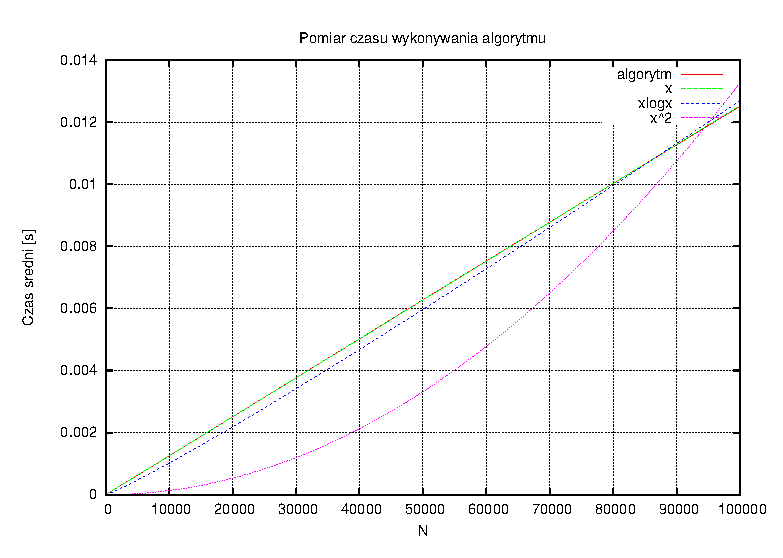
\includegraphics[width=0.8\textwidth]{wykres1.eps}
\caption{Test nr 1}
\label{Test nr 1}
\end{figure} 
\item Stos bazujący na tablicy dynamicznej, każdorazowo powiększającej swój rozmiar
\begin{figure}[!ht]
\centering
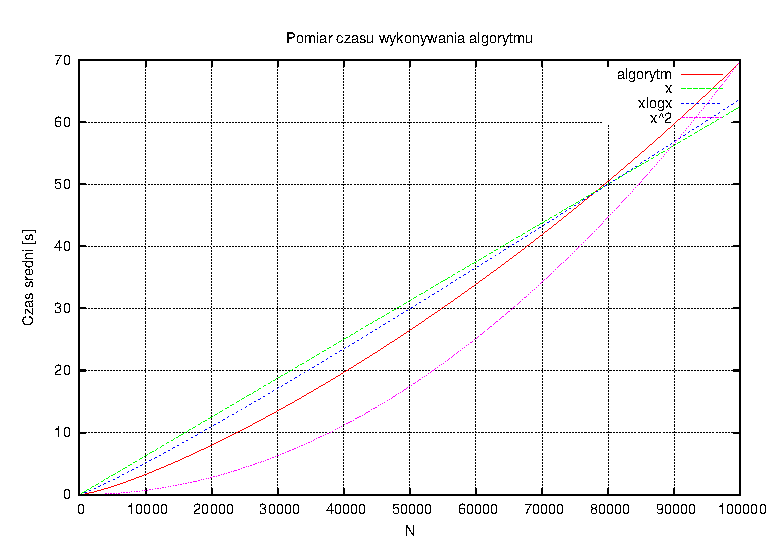
\includegraphics[width=0.8\textwidth]{wykres2.eps}
\caption{Test nr 2}
\label{Test nr 2}
\end{figure} 
\item Stos bazujący na tablicy podwajającej swój rozmiar po zapełnieniu stosu
\begin{figure}[!ht]
\centering
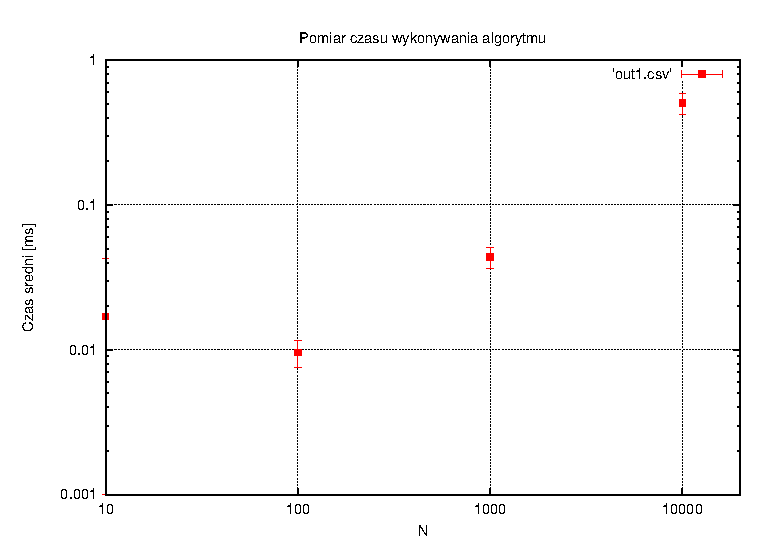
\includegraphics[width=0.8\textwidth]{wykres3.eps}
\caption{Test nr 3}
\label{Test nr 3}
\end{figure} 
\newpage
\item Kolejka bazująca na liście
\begin{figure}[!ht]
\centering
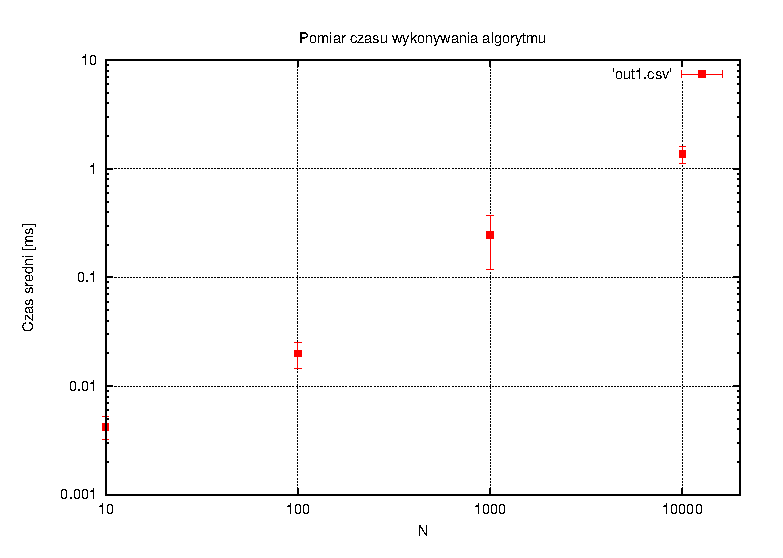
\includegraphics[width=0.8\textwidth]{wykres4.eps}
\caption{Test nr 4}
\label{Test nr 4}
\end{figure} 
\item Kolejka bazująca na tablicy każdorazowo powiększającej swój rozmiar
\begin{figure}[!ht]
\centering
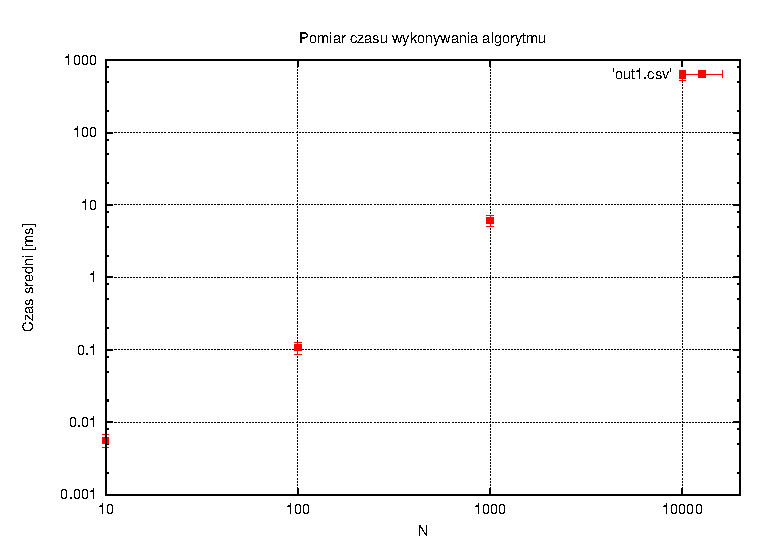
\includegraphics[width=0.8\textwidth]{wykres5.eps}
\caption{Test nr 5}
\label{Test nr 5}
\end{figure} 
\newpage
\item Kolejka bazująca na tablicy podwajającej swój rozmiar po zapełnieniu kolejki
\begin{figure}[!ht]
\centering
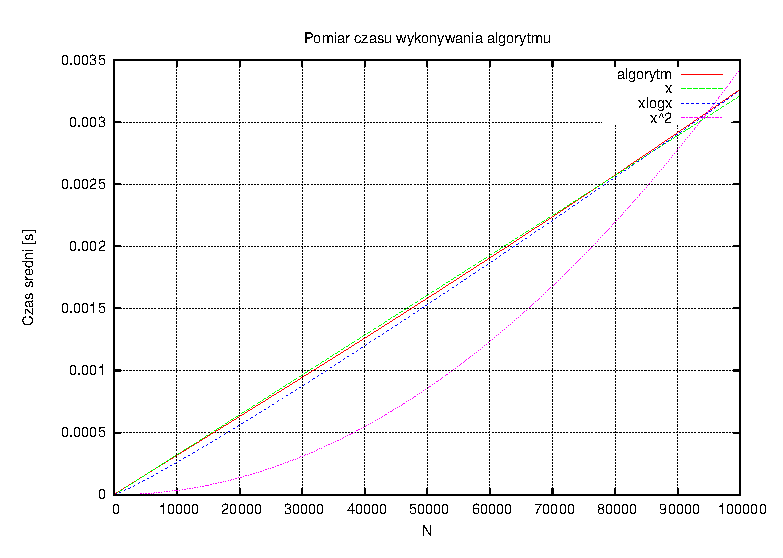
\includegraphics[width=0.8\textwidth]{wykres6.eps}
\caption{Test nr 6}
\label{Test nr 6}
\end{figure} 
\end{enumerate}

\section{Wnioski}

\begin{itemize}
\item Najbardziej wydajne pod względem szybkości wykonania okazały się struktury wykorzystujące listę lub tablicę podwajającą swój rozmiar pod wypełnieniu struktury
Złożoność obliczeniową takiej implementacji szacuje się na $ O(n) $
\item Struktury, które każdorazowo zwiększały rozmiar tablicy działają dużo wolniej, aczkolwiek są oszczędniejsze pod względem zagospodarowania pamięci.
Ich złozoność obliczeniową szacuje się na $ O(n^{2}) $
\end{itemize}
\end{document}
